\documentclass[12pt]{article}

\usepackage[a4paper, top=0.8in, bottom=0.7in, left=0.7in, right=0.7in]{geometry}
\usepackage{amsmath}
\usepackage{graphicx}
\usepackage{fancyhdr}
\usepackage{tcolorbox}
\usepackage{multicol}
\usepackage{pifont} % For checkboxes
\usepackage[defaultfam,tabular,lining]{montserrat} %% Option 'defaultfam'
\usepackage[T1]{fontenc}
\renewcommand*\oldstylenums[1]{{\fontfamily{Montserrat-TOsF}\selectfont #1}}
\renewcommand{\familydefault}{\sfdefault}
\usepackage{enumitem}
\usepackage{setspace}
\usepackage{parcolumns}
\usepackage{tabularx}
\usepackage{pgfplots} % For graph

\setlength{\parindent}{0pt}
\hyphenpenalty=10000
\exhyphenpenalty=10000

\pagestyle{fancy}
\fancyhf{}
\fancyhead[L]{\textbf{7.SL.2: Listening and Speaking}}
\fancyhead[R]{
\includegraphics[width=1cm]{Round Logo.png}}
\fancyfoot[C]{\footnotesize Study Smart Tutors}

\begin{document}

\onehalfspacing

\section*{Listening and Speaking: Text and Graph Analysis}

\textbf{Read the following texts and analyze the graph below. Then, answer the multiple-choice questions.}

\vspace{1cm}

\subsection*{Fictional Text: The Midnight Forest Adventure}

The air was thick with mystery as Lily and Max walked through the dense forest. The path ahead seemed endless, winding through trees whose branches intertwined like a tangled web. Max clutched a small flashlight in his hand, casting narrow beams of light on the darkened woods. Suddenly, Lily stopped. She thought she saw something move in the distance. "Did you see that?" she whispered to Max. Max, equally startled, nodded slowly. "I think it’s just a deer," he said, but there was uncertainty in his voice. 

The two friends continued walking cautiously, every rustle of leaves sending shivers down their spines. Their adventure in the forest was supposed to be fun, but with the moonlight barely penetrating the canopy above, it was beginning to feel more like a challenge than a game. 

Finally, they reached a clearing where a large rock jutted out from the earth. Sitting on the rock, they could see the entire forest stretching out before them, lit only by the moon. "I think we should head back," Lily said, her voice shaky. Max agreed, and they turned to make their way back home, their hearts racing from the thrill of the adventure.

\vspace{1cm}

\subsection*{Informational Text: The Role of the Moon in Earth's Ecosystem}

The moon plays an essential role in Earth's natural environment, influencing tides, stabilizing the planet's axis, and even supporting life. The gravitational pull of the moon affects the oceans, creating the ebb and flow of tides. This tidal action helps circulate ocean waters, which is vital for maintaining healthy ecosystems. Tides bring nutrients from the deep ocean to the shore, providing food for a wide variety of marine life.

The moon also helps stabilize Earth's axis, ensuring that the planet’s tilt remains consistent. This stability plays a crucial role in maintaining Earth's climate, as it prevents extreme variations in temperature. Without the moon's influence, the tilt of Earth's axis could vary significantly, leading to chaotic changes in climate.

Additionally, the moon's light has been a guiding force for humans throughout history. It has inspired art, culture, and navigation, and its influence on human activities remains a constant source of fascination.

\vspace{1cm}

\subsection*{Graph: Moonlight Intensity Throughout the Year}

Below is a graph showing the average intensity of moonlight over the course of a year. The graph shows the changes in moonlight intensity, with peaks during full moons and dips during new moons.

\begin{center}
    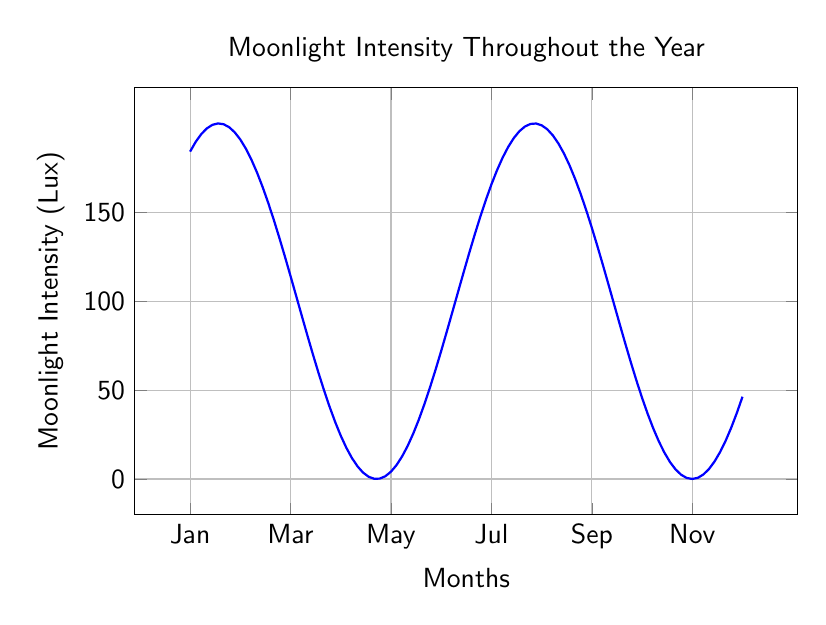
\begin{tikzpicture}
    \begin{axis}[
        title=Moonlight Intensity Throughout the Year,
        xlabel={Months},
        ylabel={Moonlight Intensity (Lux)},
        xtick={1,3,5,7,9,11},
        xticklabels={Jan, Mar, May, Jul, Sep, Nov},
        ytick={0,50,100,150},
        yticklabels={0, 50, 100, 150},
        grid=major,
        width=10cm,
        height=7cm,
        domain=1:12,
        samples=100
    ]
    % Graph showing variation in intensity
    \addplot[blue, thick] {100*sin(deg(x)) + 100};
    \end{axis}
    \end{tikzpicture}
\end{center}

\vspace{1cm}

\section*{Multiple Choice Questions}

\begin{enumerate}

\item What is the main conflict in the fictional text, "The Midnight Forest Adventure"?
\begin{enumerate}[label=\Alph*.]
    \item Lily and Max cannot find their way home.
    \item Lily and Max are lost in a forest and feel scared.
    \item Lily and Max are searching for treasure.
    \item Lily and Max are arguing about their adventure.
\end{enumerate}

\vspace{0.5cm}

\item What does Max believe the movement in the forest was?
\begin{enumerate}[label=\Alph*.]
    \item A deer
    \item A wolf
    \item A bird
    \item A bear
\end{enumerate}

\vspace{0.5cm}

\item What is the main purpose of the informational text "The Role of the Moon in Earth's Ecosystem"?
\begin{enumerate}[label=\Alph*.]
    \item To describe the importance of the moon in stabilizing Earth’s climate.
    \item To explain how the moon affects ocean tides.
    \item To discuss how the moon impacts human culture and activities.
    \item All of the above.
\end{enumerate}

\vspace{0.5cm}

\item According to the informational text, what role does the moon play in Earth’s ocean ecosystems?
\begin{enumerate}[label=\Alph*.]
    \item It helps create tides that bring nutrients to shore.
    \item It controls the temperature of the ocean.
    \item It prevents ocean water from evaporating.
    \item It causes waves to form.
\end{enumerate}

\vspace{0.5cm}

\item Which of the following is NOT mentioned as a way the moon influences Earth in the informational text?
\begin{enumerate}[label=\Alph*.]
    \item It influences ocean tides.
    \item It causes volcanic eruptions.
    \item It stabilizes Earth’s axis.
    \item It has cultural significance.
\end{enumerate}

\vspace{0.5cm}

\item How does the graph depict the intensity of moonlight over the course of the year?
\begin{enumerate}[label=\Alph*.]
    \item The intensity decreases during full moons and increases during new moons.
    \item The intensity increases during full moons and decreases during new moons.
    \item The intensity stays constant throughout the year.
    \item The intensity is highest in the middle of the year.
\end{enumerate}

\vspace{0.5cm}

\item In the graph, which month shows the highest moonlight intensity?
\begin{enumerate}[label=\Alph*.]
    \item January
    \item March
    \item July
    \item November
\end{enumerate}

\vspace{0.5cm}

\item What is the pattern shown in the graph for moonlight intensity?
\begin{enumerate}[label=\Alph*.]
    \item The intensity decreases steadily over the year.
    \item The intensity fluctuates with a peak during full moons.
    \item The intensity is highest in the spring.
    \item The intensity is highest in the fall.
\end{enumerate}

\vspace{0.5cm}

\item In the fictional text, why do Lily and Max decide to leave the forest?
\begin{enumerate}[label=\Alph*.]
    \item They are scared by the sounds of the forest.
    \item They get lost and can't find their way back.
    \item They realize it is too dark to continue.
    \item They are afraid they might encounter wild animals.
\end{enumerate}

\vspace{0.5cm}

\item According to the informational text, why is the moon’s influence on Earth’s climate important?
\begin{enumerate}[label=\Alph*.]
    \item It helps create the seasons.
    \item It stabilizes Earth’s axis, preventing extreme changes in climate.
    \item It causes the oceans to heat up.
    \item It generates wind patterns.
\end{enumerate}

\end{enumerate}

\end{document}
